\chapter{Volatility Modelling}
In this chapter, we will introduce the models to be used for option pricing in this project, namely the Heston Model and the rough Bergomi model. The Heston Model is a conventional stochastic volatility model, whereas the rough Bergomi model... 
\section{The Heston Model}
The motivation for the development of stochastic volatility models was the constant volatility assumption of the Black \& Scholes model, which proved to be incompatible with observed market option prices. Hence, stochastic volatility models must also specify the stochastics of the volatility process. One of the most popular stochastic volatility models is the Heston model, which is specified by the pair of SDEs
\begin{align}
    dS_{t}&= \mu S_{t}dt + \sqrt{\nu_{t}}S_{t}dB_{t}^{(1)},\\
    d\nu_{t}&= \kappa(\theta - \nu_{t})dt + \xi\sqrt{\nu_{t}}dB_{t}^{(2)},
\end{align}
where $\langle B^{(1)},B^{(2)}\rangle_{t}=\rho t$ with $|\rho|\leq 1$. The first SDE specifies the dynamics for the underlying asset $S_{t}$, and the second SDE is a Cox-Ingersoll-Ross process specifying the dynamics of the variance process $\nu_{t}$. Additionally, it is assumed that $S_{0},\nu_{0}>0$, and that the so-called Feller condition $2\kappa\theta >\xi^{2}$ is satisfied ensuring the variance process is strictly positive. The parameter $\theta>0$ is the long-run variance, $\kappa$ governs the speed of reversion of $\nu_{t}$ towards $\theta$, and $\xi$ is the variance of $\nu_{t}$.

For a given set of model parameters, we can simulate the paths of $S_{t}$ and $\nu_{t}$ on $[0,T]$ by the following Euler-Maruyama scheme
\begin{align}
    S_{t_{k}}^{N}&= S_{t_{k-1}}^{N} + \mu S_{t_{k-1}}^{N}\Delta_{N} + S_{t_{k-1}}^{N}\sqrt{\nu_{t_{k-1}}^{N}\left(t_{k}-t_{t_{k-1}}\right)}\zeta_{k}^{(1)}, \quad S_{0}^{N}=S_{0},\\
    \nu_{t_{k}}^{N}&= \nu_{t_{k-1}}^{N} + \kappa(\theta-\nu_{t_{k-1}}^{N})\Delta_{N} + \xi\sqrt{\nu_{t_{k-1}}^{N}\left(t_{k}-t_{t_{k-1}}\right)}\zeta_{k}^{(2)}, \quad \nu_{0}^{N}=\nu_{0},\\
\end{align}
for $N\in\N$, $\Delta_{N}=T/N$, and $k=1,\dots,N$. Furthermore
\begin{equation}
    \begin{pmatrix}
        \zeta_{k}^{(1)}\\
        \zeta_{k}^{(2)}
    \end{pmatrix} \sim \mathcal{N}(0,\Sigma),\quad \Sigma = \begin{pmatrix}
        1 & \rho \\
        \rho & 1
    \end{pmatrix}.
\end{equation}
As an example, we simulate 5 paths of $S_{t}$ and $\nu_{t}$ on the interval $[0,1]$ with 1000 points each with the following parameters.
\begin{table}[H]
\centering
\begin{tabular}{@{}lllllll@{}}
\toprule
$S_{0}$  & $\nu_{0}$   & $\mu$   & $\kappa$ & $\theta$ & $\rho$  & $\xi$ \\ \midrule
100 & 0.01 & 0.01 & 3     & 0.05  & -0.3 & 0.4   \\ \bottomrule
\end{tabular}
\caption{Parameters for Simulation.}
\label{heston_tab}
\end{table}

\begin{figure}[H]
    \centering
    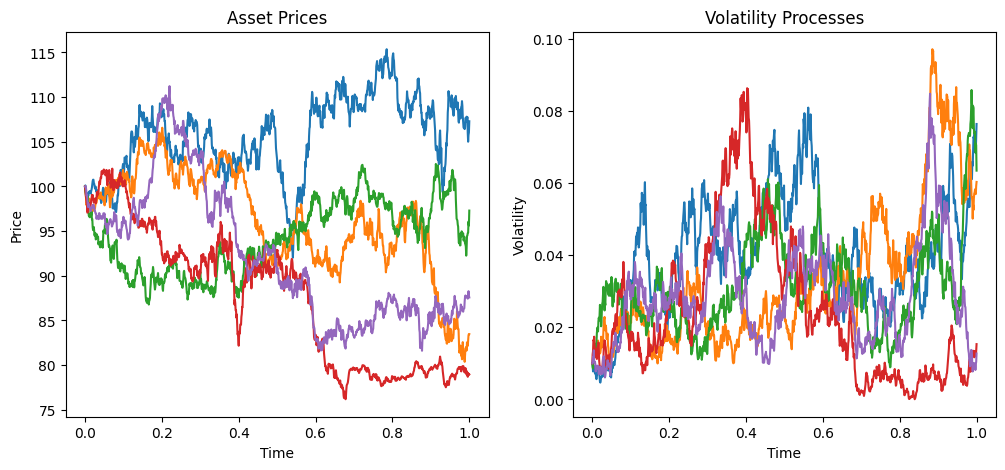
\includegraphics[scale=0.55]{fig/img/HestonModel/heston_simulations.png}
    \caption{Simulated Paths with Parameters in Table \ref{heston_tab}.}
    \label{fig:heston_simsl}
\end{figure}

%The Heston model will serve as a comparative model for our rough volatility model.
If we let $F(t,S_{t},\nu_{t})$ denote the price function of a European call option in the Heston model, then we can apply Itô's lemma and standard arbitrage arguments as in Section \ref{sec:BSM} to obtain Garman's partial differential equation
\begin{align*}
    &\frac{\partial F}{\partial t} + \frac{S_{t}^{2}\nu_{t}}{2}\frac{\partial^{2}F}{\partial S_{t}^{2}} + (r-q)S_{t}\frac{\partial F}{\partial S_{t}} - (r-q)F\\
    &+ \left(\kappa(\theta - \nu_{t})-\lambda \nu_{t}\right)\frac{\partial F}{\partial \nu_{t}} + \frac{\xi^{2}\nu_{t}}{2}\frac{\partial^{2}F}{\partial \nu_{t}^{2}} + \rho\xi S_{t}\nu_{t}\frac{\partial^{2}F}{\partial S_{t}\partial \nu_{t}}=0,
\end{align*}
where $r$ is the risk-free rate, $q$ is the dividend yield, and $\lambda$ is the market price of risk. As in the Black-Scholes model, we will assume that stocks don't pay dividens and therefore $q=0$. By analogy with the Black-Scholes formula \ref{BSFormula}, we guess a solution of the form
\begin{equation}
    F(t,S_{t},\nu_{t})=S_{t}P_{1} - e^{-r(T-t)}KP_{2},
\end{equation}
where $P_{1}$ and $P_{2}$ are the conditional risk neutral probabilities of the option expiring in the money. These probabilities are not immediately available in closed-form.
%where $P_{1}$ is the delta of the option, and $P_{2}$ is the conditional risk neutral probability of the option expiring in the money, i.e. $P_{2}=\mathbb{Q}(S_{T}>K)$ for some martingale measure $\mathbb{Q}\sim \mathbb{P}$.
However, if we let $\psi_{1},\psi_{2}$ denote the characterstic functions (Fourier transforms) of $P_{1}$ and $P_{2}$, we then have that $P_{1}$ and $P_{2}$ can be computed via the inverse Fourier transform
\begin{equation}
    P_{j}=\frac{1}{2}+\frac{1}{\pi}\int_{0}^{\infty}\textrm{Re}\left[\frac{e^{-i\phi \ln K}\psi_{j}}{i\phi}\right]d\phi, \quad j\in \{1,2\},
\end{equation}
where $i$ is the imaginary unit. Heston assumes the characteristic functions have the functional form
\begin{equation}
    \psi_{j}(\tau; \phi)=\exp\left\{C_{j}(\tau;\phi)+D_{j}(\tau;\phi)\nu_{0}+i\phi S_{0}\right\},\quad \tau=T-t, \hspace{6 pt}j\in\{1,2\}.
\end{equation}
If we substitute $\psi_{1},\psi_{2}$ into Garman's partial differential equation, we get the following ordinary differential equations for the unknown functions $C_{j}(\tau;\phi)$ and $D_{j}(\tau;\phi)$
\begin{align}
    &\frac{dC_{j}(\tau;\phi)}{d\tau}-\kappa\theta D_{j}(\tau;\phi) - r\phi i=0,\label{ode1}\\
    &\frac{dD_{j}(\tau;\phi)}{d\tau}-\frac{\xi^{2}D_{j}^{2}(\tau;\phi)}{2} + (b_{j}-\rho\xi\phi i)D_{j}(\tau;\phi) - u_{j}\phi i + \frac{\phi^2}{2}=0,\label{ode2}
\end{align}
where $j\in\{1,2\}$, and the initial conditions are $C_{j}(0;\phi)=D_{j}(0;\phi)=0$. The solution of the system \ref{ode1} - \ref{ode2} is given by
\begin{align}
    C(\tau;\phi)&=r\phi i\tau+\frac{\kappa\theta}{\xi^{2}}\left((b_{j}-\rho\xi \phi i+d)\tau -2\ln\left(\frac{1-ge^{d\tau}}{1-g}\right)\right),\\
    D(\tau;\phi)&=\frac{b_{j}-\rho\xi\phi i+d}{\xi^{2}}\left(\frac{1-e^{d\tau}}{1-ge^{d\tau}}\right),
\end{align}
where 
\begin{equation*}
    g=\frac{b_{j}-\rho\xi\phi i+d}{b_{j}-\rho\xi\phi i-d}, \quad d=\sqrt{(\rho\xi\phi i-b_{j})^{2}-\xi^{2}(2u_{j}\phi i-\phi^{2})},
\end{equation*}
with $u_{1}=1/2$, $u_{2}=-1/2$, $b_{1}=\kappa + \lambda-\rho\xi$, and $b_{2}=\kappa + \lambda$. 

As argued in \cite[p.~16]{volsurface}, we assume that the Heston process calibrated to option prices, generates the risk-neutral measure such that market price of risk $\lambda$ henceforth will be set to zero. 

\subsection{Heston Model Calibration}
Model calibration is the problem of determining the model parameters to match the market prices of a given set of options. However, in practice it is not possible nor meaningful to match the market prices exactly. Therefore, model calibration is formulated as an optimization problem, where we attempt to find the model parameters that minimize the pricing error by our model on a given set of options. One possible metric for the pricing error is the squared distance, which leads to the non-linear least squares problem
\begin{equation}\label{eq:calibration}
    \hat{\Theta}=\argmin_{\Theta}G(\Theta),\quad G(\Theta)= \sum_{i=1}^{N}w_{i}\left(F^{\Theta}_{i}(t,S_{t},T_{i},K_{i}) - F_{i}^{*}(T_{i},K_{i})\right)^{2},
\end{equation}
where $N$ is the number of options used, $w_{i}$ are weights, $F^{*}_{i}(T_{i},K_{i})$ is the market price of option $i$ with maturity time $T_{i}$ and strike price $K_{i}$, and $F^{\Theta}_{i}(t,S_{t},T_{i},K_{i})$ is the model price of the same option $i$ with model parameters $\Theta$. For the Heston model, the parameter space is $\Theta=(\nu_{0},\kappa,\theta,\xi,\rho)\subset \R^{5}$. We simply set $w_{i}=1$ for $i=1,\dots,N$ and impose the constraints on the calibrated parameters $\hat{\Theta}=(\hat{\nu}_{0},\hat{\kappa},\hat{\theta},\hat{\xi},\hat{\rho})$ that $\hat{\nu}_{0}\in [0.001, 0.25]$, $\hat{\kappa}\in [0.001, 5]$, $\hat{\theta}\in [0.001, 0.1]$, $\hat{\xi}\in [0.01, 1]$, and $\hat{\rho}\in [-0.99, 0.99]$ with initial guesses $\hat{\Theta}_{0}=(0.1, 3, 0.05, 0.3, -0.8)$. Additionally, we set to the tolerance for termination to $0.001$, and we use an extension of the limited-memory BFGS algorithm, which can handle the box constraints imposed on the parameters, to solve the optimization problem \eqref{eq:calibration}.
%Applying Itô's lemma and standard arbitrage arguments as in Section \ref{sec:BSM}, we obtain the 
\section{Fractional Ornstein-Uhlenbeck Process}
The rough fractional stochastic volatility (RFSV) model that we will consider in the subsequent section, models the volatility process via the fractional Ornstein-Uhlenbeck process, which is given by the SDE
\begin{align}
    dY_{t}&= -\alpha(Y_{t}-m)dt + \varphi dB^{H}_{t},\quad 0\leq t\leq T,
\end{align}
where $m \in \R$, $\alpha,\varphi >0$, and $B^{H}$ is a fBM of Hurst index $H\in(0,1/2)$, which is where the "rough" nomenclature stems from. The volatility process $\sigma = (\sigma_{t})_{0\leq t\leq T}$ is then modelled by $\sigma_{t}= e^{Y_{t}}$. As for the usual Ornstein-Uhlenbeck process, there is an explicit form for the solution
\begin{equation}\label{ornstein_sol}
    Y_{t}= m + (Y_{0}-m)e^{-\alpha t} + \varphi e^{-\alpha t}\int_{0}^{t}e^{\alpha s}dB_{s}^{H}.
\end{equation}
The integral in \eqref{ornstein_sol} can in accordance with Proposition \ref{thm:integration} be calculated as the pathwise Riemann-Stieltjes integral
\begin{equation}\label{eq:riemann}
    \int_{0}^{t}e^{\alpha s}dB_{s}^{H}=\lim_{N\to\infty}\sum_{k=0}^{N-1}e^{\alpha k t/N}\left(B_{(k+1)t/N}^{H}-B_{kt/N}^{H}\right).
\end{equation}
Thus, for $N\in\N$ sufficiently large, the above Riemann-sum will approximate the integral in \eqref{ornstein_sol} well. Changing the summation index in \eqref{eq:riemann}, we introduce the quantity
\begin{equation}
    \mathbb{B}_{t}^{H,N}\coloneqq \sum_{l=1}^{\lfloor Nt\rfloor }e^{\alpha l/N}\left(B^{H}_{l/N}-B^{H}_{(l-1)/N}\right)
\end{equation}
Thus, we can simulate a fractional Ornstein-Uhlenbeck process on the grid $0=t_{0}<t_{1}<\dots<t_{N}=T$ by the following scheme
\begin{equation}\label{fou_exact}
    Y_{t_{j}}^{N}=m + (Y_{0}-m)e^{-\alpha t_{j}} + \varphi e^{-\alpha t_{j}}\mathbb{B}_{t_{j}}^{H,N},\quad Y_{0}^{N}=Y_{0}, \quad j=1,\dots,N.
\end{equation}
Alternatively, we could use the Euler-Maruyama scheme to simulate the process
\begin{equation}\label{fou_euler}
    Y_{t_{j}}^{N}=Y_{t_{j-1}} -\alpha(Y_{t_{j-1}}-m)\Delta_{N} + \varphi\Delta B_{t_{j-1}}^{H},\quad Y_{0}^{N}=Y_{0},\quad j=1,\dots,N,
\end{equation}
where $\Delta_{N}=T/N$ and $\Delta B_{t_{j}}^{H}=B^{H}_{t_{j}}-B^{H}_{t_{j-1}}$. The error rates for the two simulation methods in \eqref{fou_exact} and \eqref{fou_euler} are approximately the same, and since the Euler-Maruyama scheme is computationally faster, we will use the methodology in \eqref{fou_euler} for simulation.

As an example, if we take the process with $H=0.2$, $\alpha = 1$, $m=1$, $\varphi=1/2$, and $Y_{0}=0$, i.e.
\begin{equation}
    dY_{t}=-(Y_{t}-1)dt+\frac{1}{2}dB^{0.2}_{t},\quad Y_{0}=0,
\end{equation}
and use \eqref{fou_exact} with $N=100,000$ as our true solution path $Y_{t}$, then we can compare the Euler-approximations. This comparison is seen in Figure \ref{fig:euler-scheme}, where the true solution path is plotted with the Euler-approximations superimposed. It is seen that for $N\geq 1000$, the true solution is approximated well by the Euler scheme.
\begin{figure}[H]
    \centering
    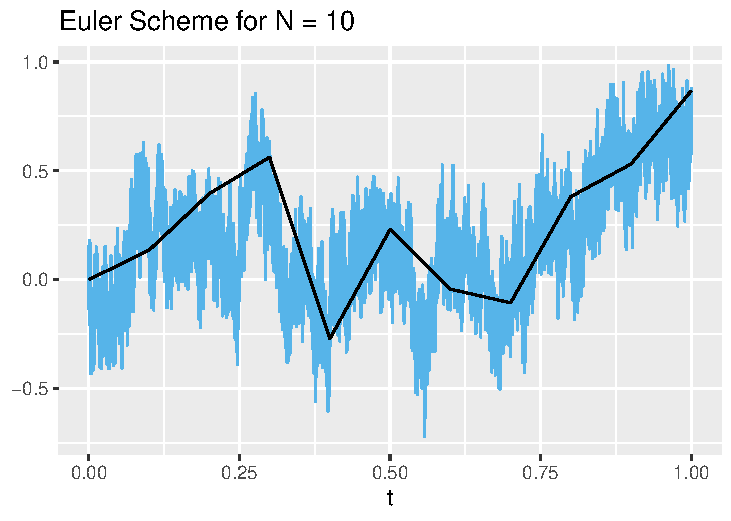
\includegraphics[scale=0.52]{fig/img/EulerScheme/EulerScheme10.pdf}
    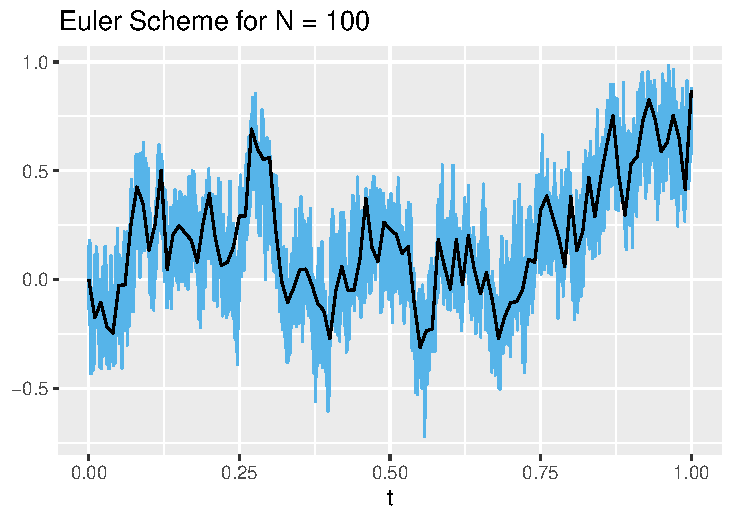
\includegraphics[scale=0.52]{fig/img/EulerScheme/EulerScheme100.pdf}
    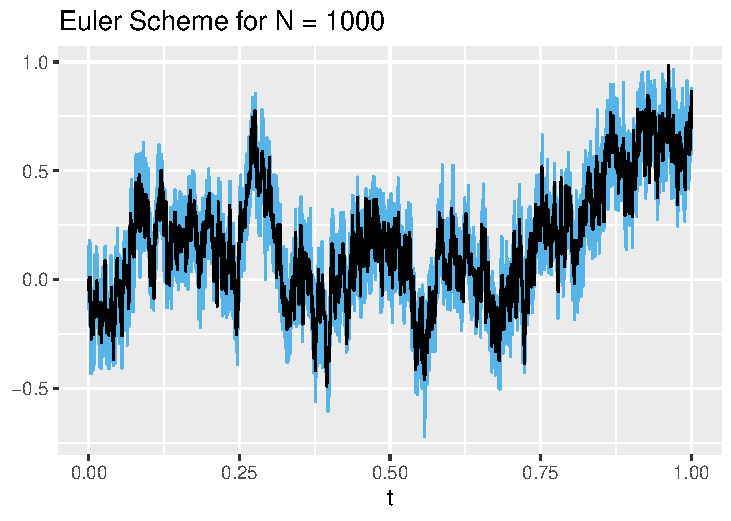
\includegraphics[scale=0.52]{fig/img/EulerScheme/EulerScheme1000.pdf}
    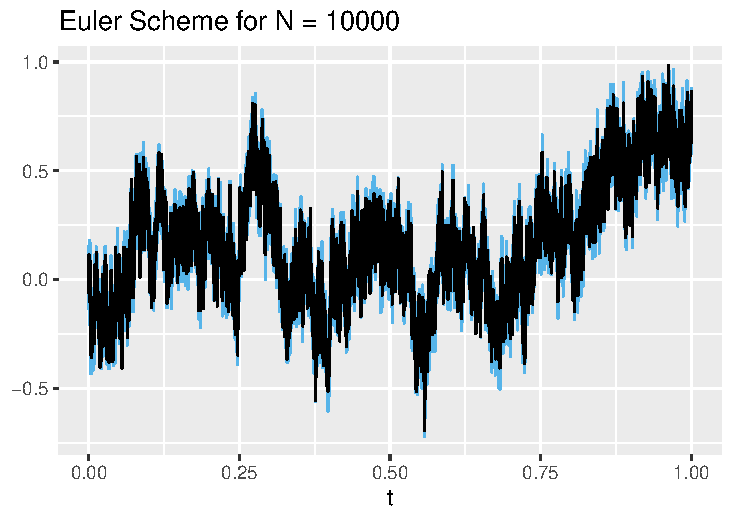
\includegraphics[scale=0.52]{fig/img/EulerScheme/EulerScheme10000.pdf}
    \caption{Euler Approximations for Various Step Sizes $\Delta_{N}$. }
    \label{fig:euler-scheme}
\end{figure}

\section{Volatility is Rough}
This section is based on \cite{volisrough}.

In this section, we will use the methodology presented in \cite{volisrough} to argue that the volatility process of financial time series is indeed rough and estimate the roughness of the volatility process. Suppose we have discrete observations of the volatility process $\sigma$ on the interval $[0,T]$ with mesh size $\Delta$, i.e. $\sigma_{0},\sigma_{\Delta},\dots,\sigma_{N\Delta}$ with $N\coloneqq \lfloor T/\Delta\rfloor$. Then for $q\geq 0$, we define the statistic
\begin{equation}\label{eq:mstat}
    m(q,\Delta)\coloneqq \frac{1}{N}\sum_{k=1}^{N}|\log(\sigma_{k\Delta})-\log(\sigma_{(k-1)\Delta})|^{q}.
\end{equation}
It is assumed that for some $s_{q}>0$ and $b_{q}>0$, we have
\begin{equation}\label{weirdlim}
    N^{qs_{q}}m(q,\Delta)\to b_{q}\quad \textrm{as}\quad \Delta\to 0^{+}.
\end{equation}
Under additional technical conditions, $s_{q}$ can be viewed as the regularity of the volatility. In particular, a function satisfying \eqref{weirdlim} is Hölder continuous with Hölder exponent $\alpha$ for any $\alpha <s_{q}$. For instance, if $\log(\sigma_{t})$ was a fBM with Hurst index $H$, then \eqref{weirdlim} would hold in probability with $s_{q}=H$ for any $q\geq 0$. Assuming the increments of the log-volatility process are stationary and that a law of large numbers can be applied, \eqref{eq:mstat} can be seen as the empirical counterpart of 
\begin{equation}
    \E\left[|\log(\sigma_{\Delta})-\log(\sigma_{0})|^{q}\right].
\end{equation}

To estimate the smoothness parameter $s_{q}$ for each $q$, we compute $m(q,\Delta)$ for different $\Delta$ and regress $\log(m(q,\Delta))$ against $\log(\Delta)$. Since the volatility process is not directly observable, we have to proxy the true spot volatility. For this purpose, we use the daily realized variance estimates of the Oxford-Man Institute of Quantitative Finance Realized Library as our proxy for daily spot variance. The daily realized variance is calculated using intradaily intervals of 5 minutes over the 8 hour trading day of the S\&P-500 index. The data starts at 1/3-2000 and ends at 3/31-2020 totalling 5079 trading days. A plot of the data is seen in Figure \ref{fig:realized} along with the realized volatility (square root of the realized variance estimates).

%\begin{figure}[H]
%    \centering
%    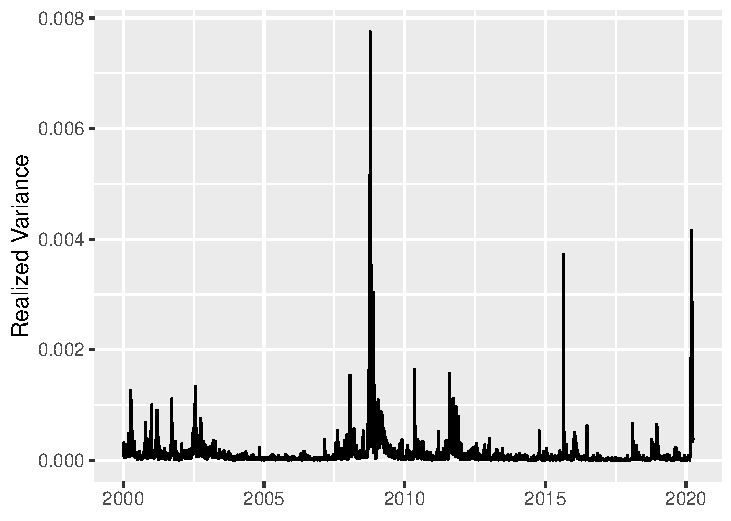
\includegraphics[scale=0.6]{fig/img/RealizedLib/SP500Realized.pdf}
%    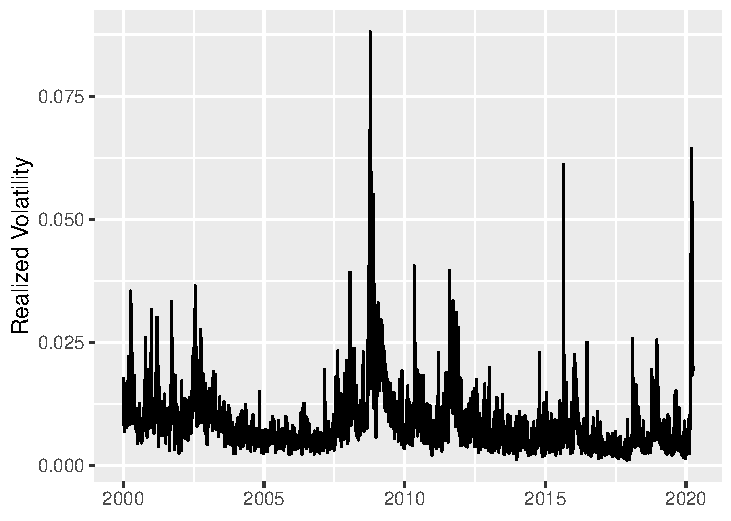
\includegraphics[scale=0.6]{fig/img/RealizedLib/SP500RealizedVol.pdf}
%    \caption{Realized Variance (left) and Volatility (right) of the S\&P-500.}
%    \label{fig:realized}
%\end{figure}
\begin{figure}[H]
    \centering
    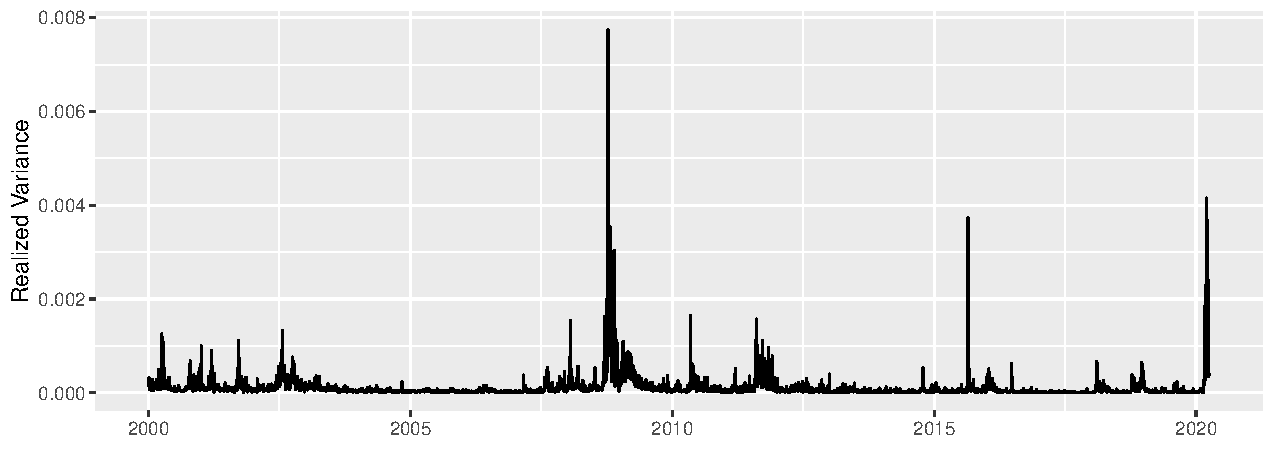
\includegraphics[scale=0.6]{fig/img/RealizedLib/realized_variance_longplot.pdf}
    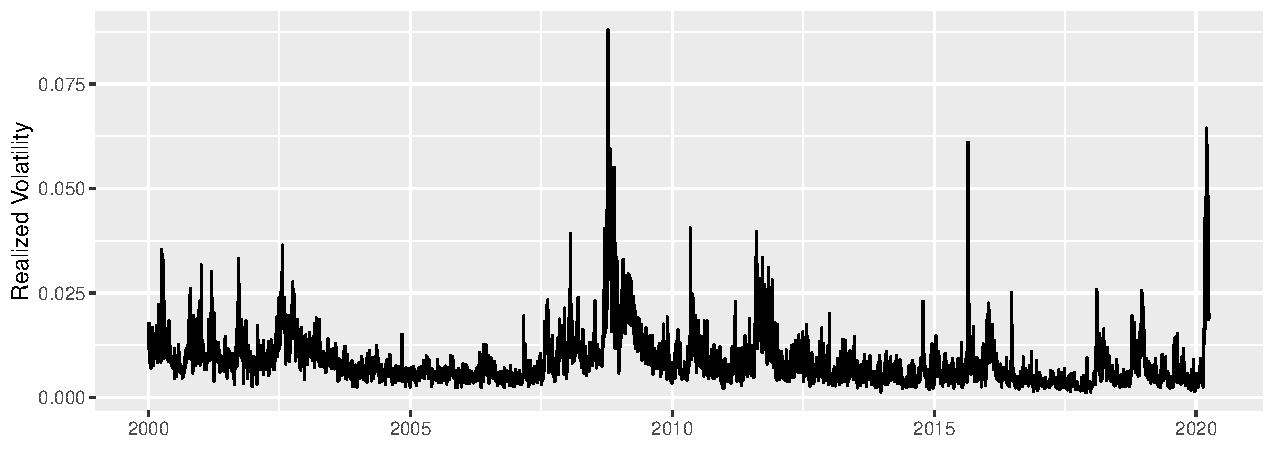
\includegraphics[scale=0.6]{fig/img/RealizedLib/realized_volatility_longplot.pdf}
    \caption{Realized Variance (top) and Realized Volatility (bottom) of the S\&P-500.}
    \label{fig:realized}
\end{figure}
We proceed to compute $m(q,\Delta)$ for $q\in \{0.5,1,1.5,2,3\}$ and $\Delta \in \{1,2,\dots,30\}$, and regress $\log m(q,\Delta)$ against $\log\Delta$. As seen in Figure \ref{fig: Linear_reg}, the points lie very close to the regression line for each value of $q$.
\begin{figure}[H]
    \centering
    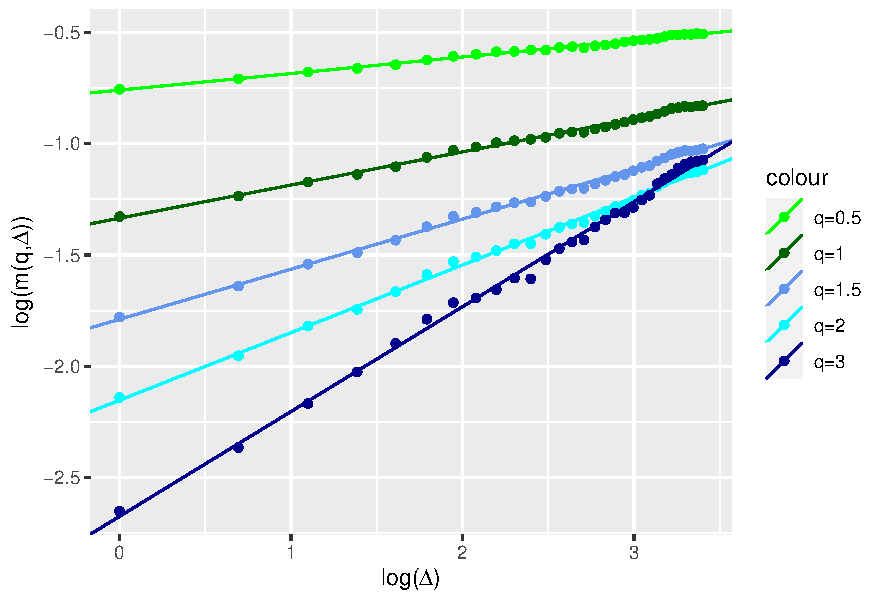
\includegraphics[scale=0.8]{fig/img/RealizedLib/Linear_Reg_rigtig.pdf}
    \caption{$\log m(q,\Delta)$ as a function of $\log\Delta$, S\&P-500.}
    \label{fig: Linear_reg}
\end{figure}
 If we assume stationarity of the log-volatility process, then the linear relationship in Figure \ref{fig: Linear_reg} implies the following scaling property in expectation
 \begin{equation}\label{eq:scaling}
     \E[|\log(\sigma_{\Delta})-\log(\sigma_{0})|^{q}]=K_{q}\Delta^{\zeta_{q}},
 \end{equation}
 where $\zeta_{q}>0$ is the slope of the regression line associated to $q$. The log-log plot in Figure \ref{fig: Linear_reg} establishes that $m(q,\Delta)\hspace{2 pt}\propto\hspace{2 pt} \Delta^{\zeta_{q}}$ for each $q$, and we now turn to how $\zeta_{q}$ scales with $q$. From Figure \ref{fig:slope_plot}, we find the monofractal scaling relationship $\zeta_{q}=qH$, i.e. $\zeta_{q}$ and $q$ are proportional. In Figure \ref{fig:slope_plot}, we have plotted the best straight line fit (blue) along with the line $q\mapsto 0.15183\cdot q$ (black). The two lines are hardly distinguishable, and therefore the estimated smoothness is $H=0.15183$. 
 \begin{figure}[H]
     \centering
     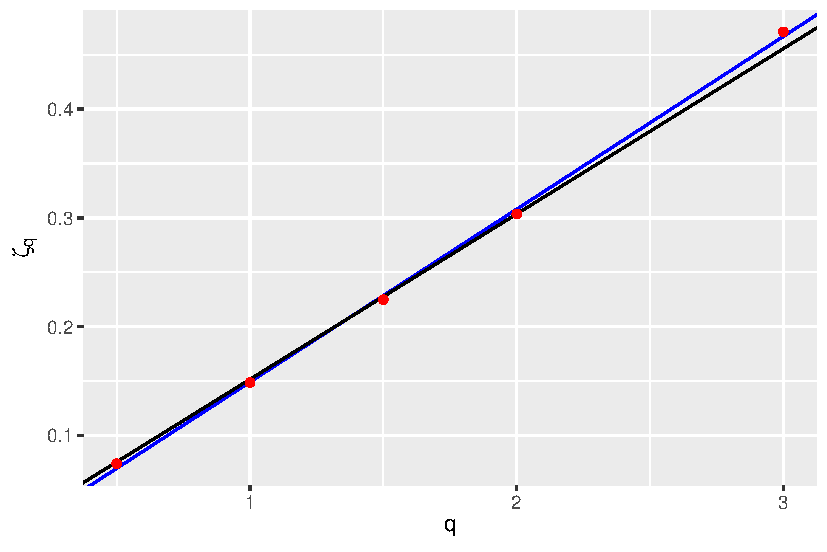
\includegraphics[scale=0.75]{fig/img/RealizedLib/slope_plot.pdf}
     \caption{Scaling of $\zeta_{q}$ with $q$.}
     \label{fig:slope_plot}
 \end{figure}
 Hence, we have obtained a methodology for measuring the smoothness parameter $s_{q}=H$ by taking $\hat{H}=\zeta_{q}/q$. In Figure \ref{fig: Linear_reg}, we computed the slopes $\zeta_{q}$ for $q\in\{0.5,1, 1.5,2,3\}$, and therefore obtain the estimates
 \begin{table}[H]
\centering
\begin{tabular}{@{}llllll@{}}
\toprule
$q$  & $0.5$   & $1$   & $1.5$ & $2$ & $3$ \\ \midrule 
$\zeta_{q}$ & 0.07435 & 0.14885 & 0.22498     & 0.30365  & 0.47087 \\  \midrule
$\hat{H}$ & 0.14870 & 0.14885 & 0.14999 & 0.15183 & 0.15696 \\ \bottomrule
\end{tabular}
\caption{Estimated smoothness $\hat{H}$ for different $q$.}
\label{heston_tab}
\end{table}
In Figure \ref{fig:slope_plot}, the estimate $\hat{H}=0.15183$ was used, since this gave the best fit to the blue regression line.
 %As shown in \cite{volisrough}, the slope $\zeta_{q}$ is approximately directly proportional to the smoothness parameter $s_{q}$, i.e. $\xi_{q}\approx qs_{q}$. 
 
 The increments of a fBM $\Delta B_{t}^{H}=B_{t+\Delta}^{H}-B_{t}^{H}$ is a centered Gaussian with variance $\Delta^{2H}$. Thus, we obtain that its absolute moments satisfy 
 \begin{equation}
     \E\left[|B^{H}_{t+\Delta}-B_{t}^{H}|^{q}\right]=K_{q}\Delta^{\zeta_{q}},
 \end{equation}
 where $K_{q}$ is the $q$'th absolute moment of a standard Gaussian variable and $\zeta_{q}=qH$. Hence, the fractional Brownian motion $B^{H}$ also satisfies the scaling property \eqref{eq:scaling}. Consequently, the fBM seems like a good choice as a model for the log-volatility process based on the above discussion.
 
 Having established the scaling property in \eqref{eq:scaling}, we now turn to the distribution of the increments of the log-volatility. It is a well-established stylized fact that the distribution of increments of log-volatility is close to Gaussian (see e.g. \cite{bollerslev}), which is also validated in Figure \ref{fig:histograms} for the S\&P-500, where the Gaussian distribution seems to hold for any lag $\Delta$. The fitted normal density $\hat{f}\sim \mathcal{N}(\hat{\mu}, \hat{\sigma})$ with the sample mean and sample standard deviation as parameters is also superimposed in red.
 \begin{figure}[H]
    \centering
    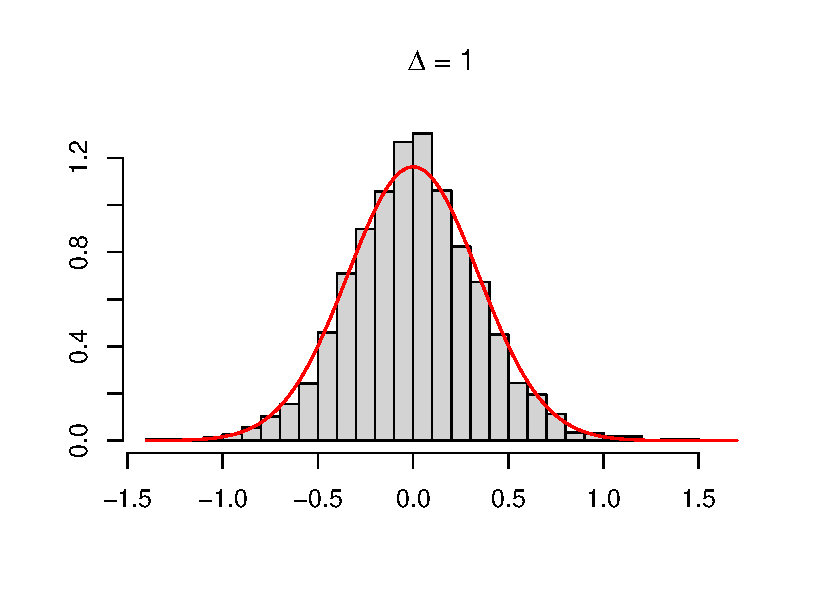
\includegraphics[scale=0.5, width = 7cm]{fig/img/RealizedLib/histograms/histogram1.pdf}
    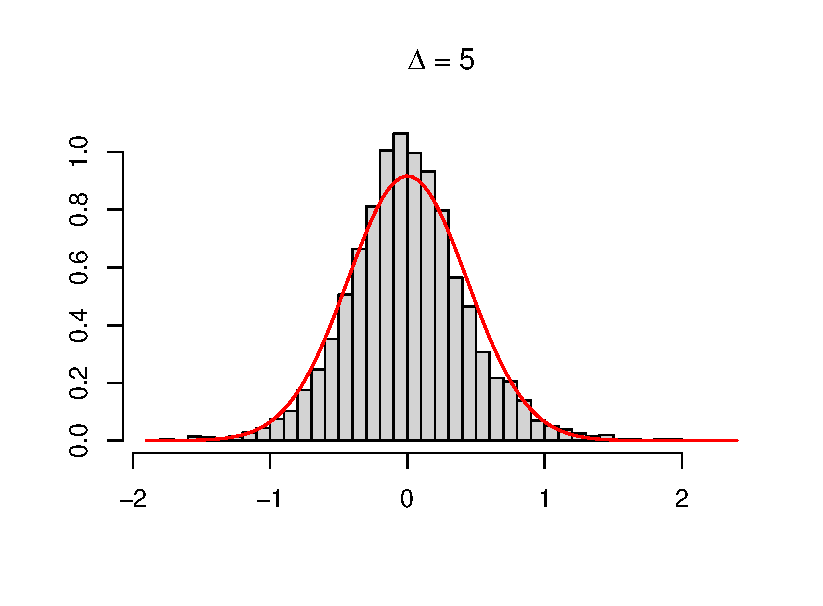
\includegraphics[scale=0.5, width = 7cm]{fig/img/RealizedLib/histograms/histogram5.pdf}\hfill
    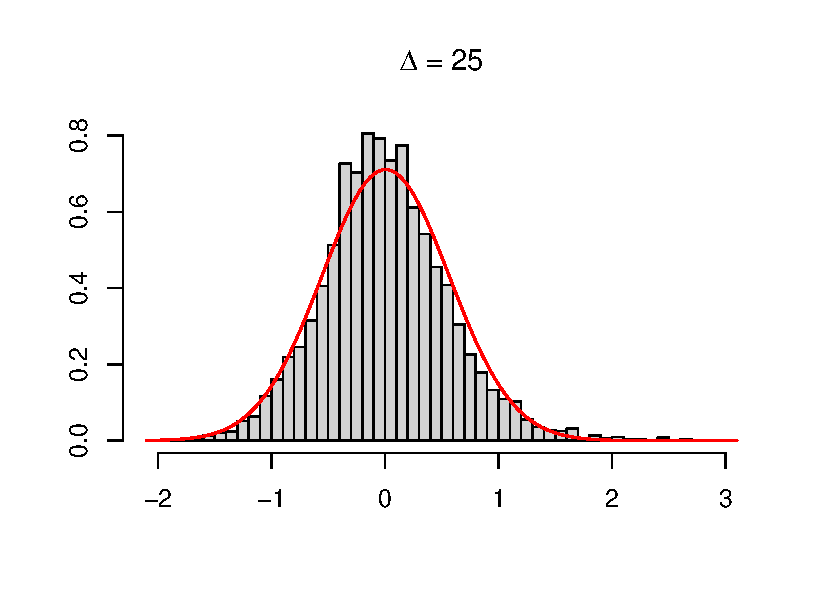
\includegraphics[scale=0.5, width = 7cm]{fig/img/RealizedLib/histograms/histogram25.pdf}
    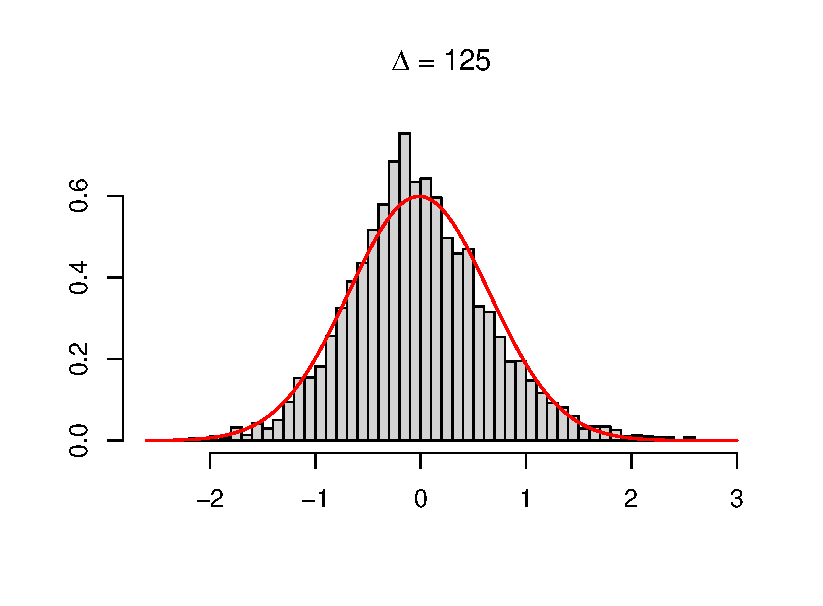
\includegraphics[scale=0.5, width = 7cm]{fig/img/RealizedLib/histograms/histogram125.pdf}
    \caption{Histograms for different lags $\Delta$ of increments $\log\sigma_{t+\Delta}-\log\sigma_{t}$, S\&P-500.}
    \label{fig:histograms}
\end{figure}
In conclusion, the preceding discussion would seem to suggest a model of the form
\begin{equation}\label{eq:simple_model}
    \log \sigma_{t+\Delta} - \log \sigma_{t} = \varphi(B^{H}_{t+\Delta}-B^{H}_{t}),
\end{equation}
where $\varphi >0$ is a positive constant, and $B^{H}$ is a fractional Brownian motion with Hurst index $H$ equal to the measured smoothness $s_{q}$ of the process. The model \eqref{eq:simple_model} can be rewritten as 
\begin{equation}
    \sigma_{t}=\sigma \exp\left(\varphi B_{t}^{H}\right),
\end{equation}
where $\sigma$ is another positive constant. However, this model is not stationary, which implies that the volatility in theory could grow infinitely large. Stationarity is imposed by modelling the log-volatility as a fractional Ornstein-Uhlenbeck process. Hence, we arrive at the rough volatility model suggested in the previous section
\begin{align}
    dY_{t}&= -\alpha(Y_{t}-m)dt + \varphi dB^{H}_{t},\\
    \sigma_{t} &= e^{Y_{t}},
\end{align}
where $\alpha,\varphi>0$, $m\in \R$, and $H\in (0,1/2)$.
\subsection{Estimation of Parameters}
We now turn to the problem of estimating the parameters for a fractional Ornstein-Uhlenbeck process $Y$, if we have a discrete sample $Y_{i\Delta}$, where $i=0,1,\dots,N$ and $\Delta>0$. We propose a two-stage estimation approach, where the first stage consists of estimating $H$ by using the change-of-frequency estimator based on the second-order differences of $Y$. Based on the estimator of $H$, we then obtain a plug-in estimator of $\varphi$. In the second stage, we esimate $m$ and $\alpha$ by using method-of-moments estimators. 

For estimating the Hurst index $H$, we make use of the following result derived in \cite{barndorff}. It states that for fixed $T>0$ and $N\coloneqq \lfloor T/\Delta\rfloor$, we have
\begin{equation}
    \frac{\sum_{i=4}^{N}|Y_{i\Delta}-2Y_{(i-2)\Delta}+Y_{(i-4)\Delta}|^{2}}{\sum_{i=2}^{N}|Y_{i\Delta}-2Y_{(i-1)\Delta}+ Y_{(i-2)\Delta}|^{2}}\overset{\mathbb{P}}{\to} 2^{2H}\quad \textrm{as}\quad \Delta\to 0^{+}.
\end{equation}
Naturally, this leads us to the change-of-frequency (COF) estimator
\begin{equation}
    \hat{H}=\frac{1}{2}\log_{2}\left(\frac{\sum_{i=4}^{N}|Y_{i\Delta}-2Y_{(i-2)\Delta}+Y_{(i-4)\Delta}|^{2}}{\sum_{i=2}^{N}|Y_{i\Delta}-2Y_{(i-1)\Delta}+ Y_{(i-2)\Delta}|^{2}}\right).
\end{equation}
Based on the estimator of $H$, we can obtain a plug-in estimator of $\varphi$ using the quadratic variation of the second-order difference, i.e.
\begin{equation}
    \hat{\varphi} = \sqrt{\frac{\Delta}{T\tau}\sum_{i=2}^{N}|Y_{i\Delta}-2Y_{(i-1)\Delta}+ Y_{(i-2)\Delta}|^{2}},
\end{equation}
where $\tau = 4\Delta^{2\hat{H}}-(2\Delta)^{2\hat{H}}$. 

Since $\alpha>0$, $Y$ is both stationary and ergodic, which means that we can use functions of the sample moments $\frac{1}{N}\sum_{i=0}^{N}Y_{i\Delta}$ and $\frac{1}{N}\sum_{i=0}^{N}Y_{i\Delta}^{2}$ to estimate $\alpha$ and $m$. Based on the estimators of $H$ and $\varphi$, we define the moment estimators
\begin{align}
    \hat{m} &= \frac{1}{N}\sum_{i=0}^{N}Y_{i\Delta},\\
    \hat{\alpha} &= \left(\frac{N\sum_{i=0}^{N}Y_{i\Delta}^{2}-\left(\sum_{i=0}^{N}Y_{i\Delta}\right)^{2}}{N^{2}\hat{\varphi}^{2}\hat{H}\Gamma(2\hat{H})}\right)^{-1/2\hat{H}},
\end{align}
where $\Gamma: (0,\infty)\to (0,\infty)$ denotes the gamma function.

If we use the estimators defined above on our data with $\Delta=1$ (for 1 trading day) and $N=5079$, we can simulate a path of the volatility process $\sigma_{t}=\exp(Y_{t})$. Our estimated parameter values are $\hat{H}=0.128$, $\hat{\varphi}=0.842$, $\hat{m} = -4.95$, and $\hat{\alpha} = 0.05$.
\begin{figure}[H]
    \centering
    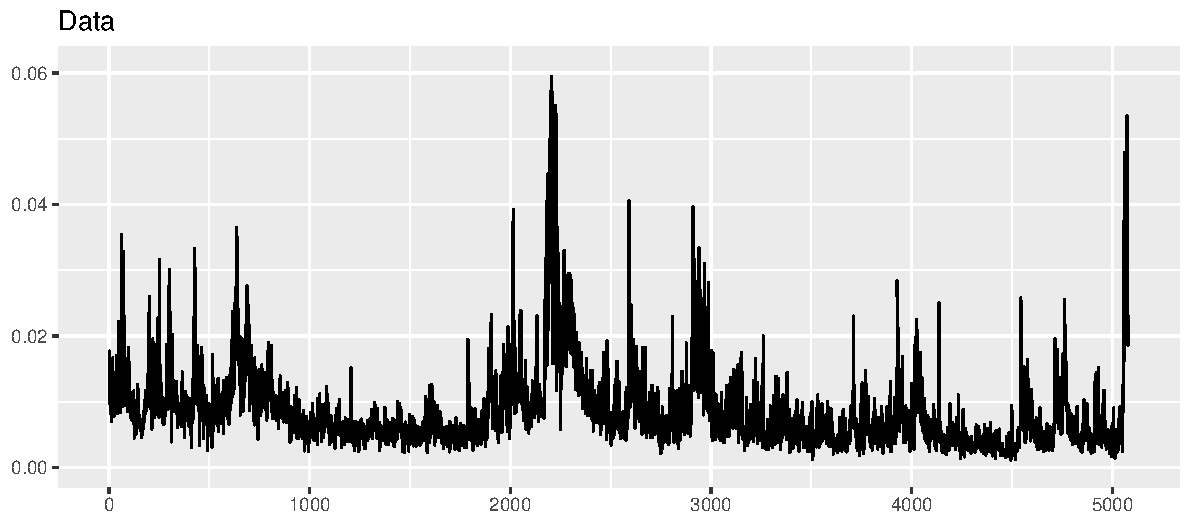
\includegraphics[scale=0.65]{fig/img/RealizedLib/RealizedVolWithoutDates.pdf}
    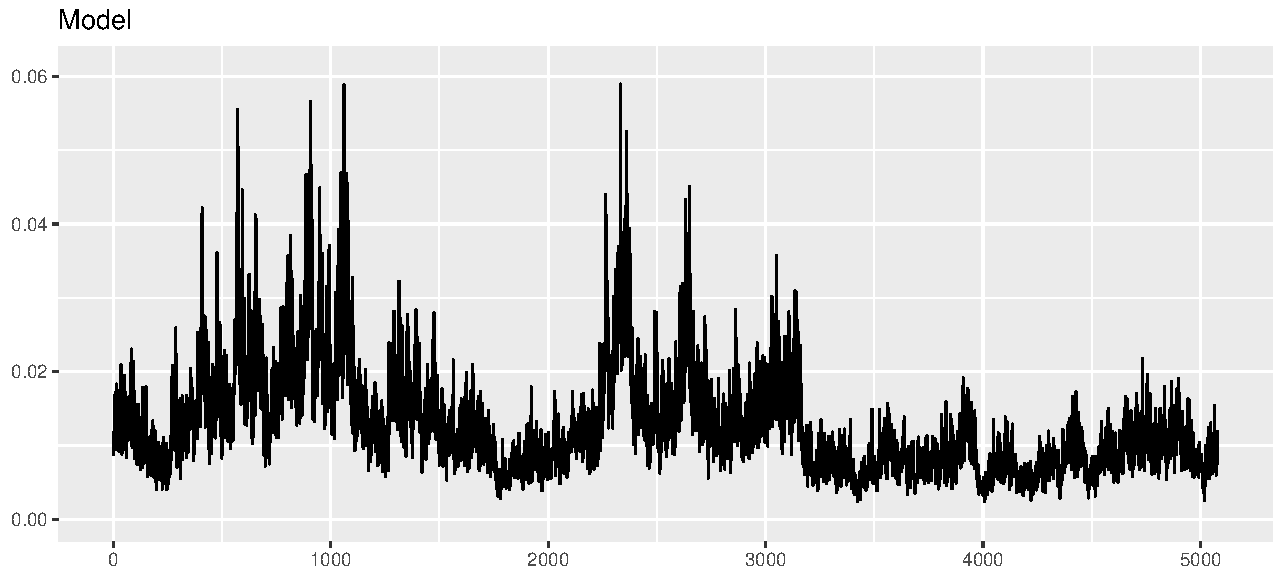
\includegraphics[scale=0.6]{fig/img/RealizedLib/simulated_vol_ny.pdf}
    \caption{Volatility of S\&P-500 (top) and of the model (bottom).}
    \label{fig:datavol_modelvol}
\end{figure}
All of the estimators turn out to be consistent and have tractable asymptotic distributions. Since we will mainly focus on the estimation of the roughness parameter $H$, we will only present results for $\hat{H}$.
\begin{thm}\label{thm:asymp}
    Let $H\in (0,1)$ and $T>0$ be fixed and set $N\coloneqq T/\Delta$. Then as $\Delta\to 0^{+}$, we have $\hat{H}\overset{\mathbb{P}}{\to} H$ and 
    \begin{equation}
        \sqrt{N}(\hat{H}-H)\overset{d}{\to}\mathcal{N}\left(0,\frac{\Sigma_{11}+\Sigma_{22}-2\Sigma_{12}}{(2\log 2)^2}\right),
    \end{equation}
    where 
    \begin{align}
        \Sigma_{11} &\coloneqq 2 + 2^{2-4H}\sum_{j=1}^{\infty}\left(\rho_{j+2}+4\rho_{j+1}+6\rho_{j} + 4\rho_{|j-1|}+ \rho_{|j-2|}\right)^{2},\\
        \Sigma_{12}&\coloneqq 2^{1-2H}\left(4(\rho_{1}+1)^{2}+2\sum_{j=0}^{\infty}(\rho_{j+2}+2\rho_{j+1}+\rho_{j})^{2}\right),\\
        \Sigma_{22}&\coloneqq 2+4\sum_{j=1}^{\infty}\rho_{j}^{2},
    \end{align}
with 
\begin{equation}
    \rho_{j}\coloneqq \frac{1}{2(4-2^{2H})}\left(-|j+2|^{2H} + 4|j+1|^{2H} - 6|j|^{2H} + 4|j-1|^{2H} - |j-2|^{2H}\right).
\end{equation}
\end{thm}
We will only apply Theorem \ref{thm:asymp} and not prove it. Note that although, we are only interested in $H<1/2$, the asymptotics of $\hat{H}$ apply to all $H\in (0,1)$.
\begin{figure}[H]
    \centering
    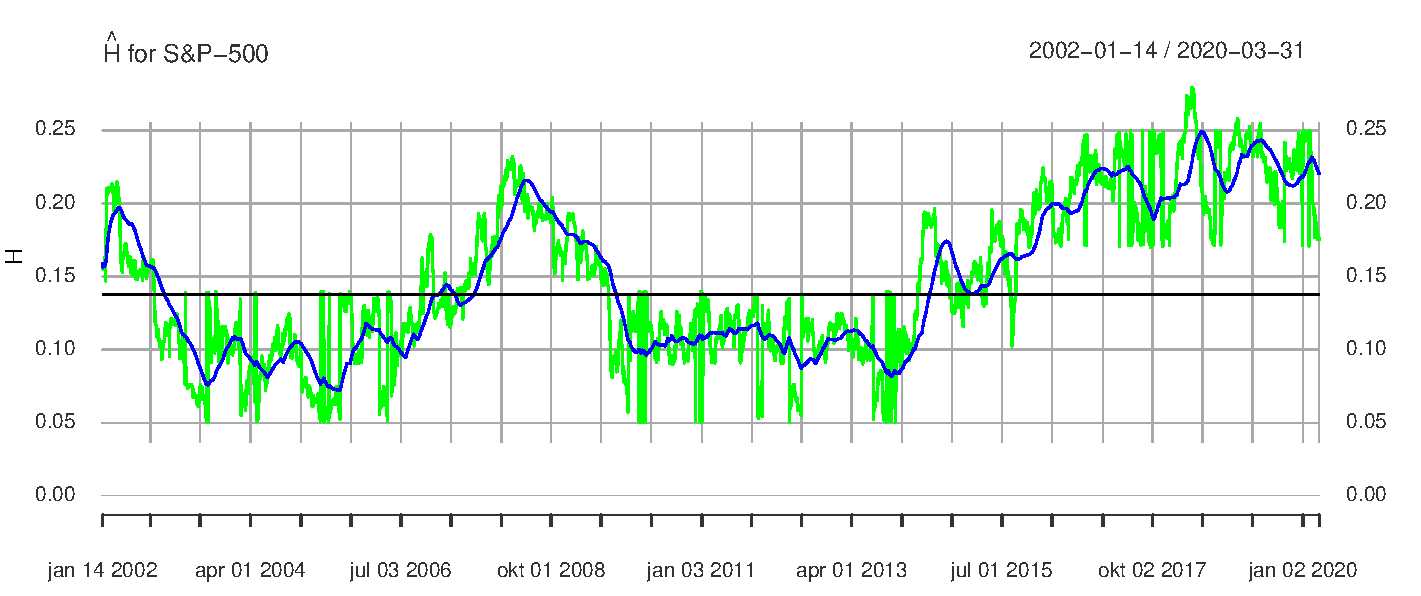
\includegraphics[scale=0.65]{fig/img/RealizedLib/rolling_H.pdf}
    \caption{Caption}
    \label{fig:enter-label}
\end{figure}
%For our rough stochastic volatility model, the underlying asset $S_{t}$ follows the SDE
%\begin{equation}
%    dS_{t}=\mu_{t}S_{t}dt + \sigma_{t}S_{t}dB_{t},
%\end{equation}
%where $\mu_{t}$ is the drift process, which may be deterministic, and $\sigma_{t}$ is the volatility process. The volatility process satisfies 
%\begin{align}
%    dY_{t}&= -\lambda(Y_{t}-\theta)dt + \varphi dB^{H}_{t}\\
%    \sigma_{t} &= e^{Y_{t}},
%\end{align}
%where $\theta\in \R$ and $\lambda,\varphi >0$.